% !TEX encoding = UTF-8 Unicode
% !TEX program = xelatex

\documentclass{article}
	\usepackage[margin=1in]{geometry}
	\usepackage{tikz}
	\usepackage{listings}
	\usepackage{xeCJK}
		\setmainfont{SourceCodePro-Regular}
		\setCJKmainfont{NotoSansTC-Regular}
\begin{document}



	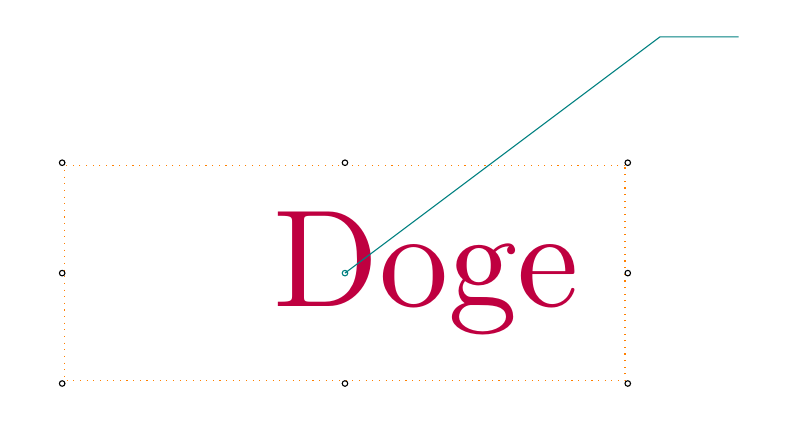
\begin{tikzpicture}\setmainfont{NotoSansTC-Regular}
		\path (0, 0) node (Doge)
			[scale = 5, draw=orange, dotted, text=purple]
				{煮豆燃 Doge};
		\draw (Doge.north)      circle(1pt) node[above] {北};
		\draw (Doge.north east) circle(1pt) node[above right] {東北};
		\draw (Doge.east)       circle(1pt) node[right] {東};
		\draw (Doge.south east) circle(1pt) node[below right] {東南};
		\draw (Doge.south)      circle(1pt) node[below] {南};
		\draw (Doge.south west) circle(1pt) node[below left] {西南};
		\draw (Doge.west)       circle(1pt) node[left] {西};
		\draw (Doge.north west) circle(1pt) node[above left] {西北};
		\draw (Doge.center)     circle(1pt)
			-- ++(4, 3) -- ++(1, 0) [teal] node[right] {中心};
	\end{tikzpicture}



\lstset{
	language=[latex]tex,tabsize=4,
	moredelim=*[s][\itshape]{$}{$},
	moredelim=*[s][\color{red!40!.}]{(}{)},
	moredelim=*[s][\color{green!30!.}]{[}{]},
	backgroundcolor=\color{blue!5},
	commentstyle=\color{.!80}\itshape,
	texcsstyle=*\color{blue!40!.},
	moretexcs={
		setmainfont,
		draw,path
	},
	deletetexcs={},
}
%%%%%%%%%%%%%%%%%%%%%%%%%%%%%%%%%%%%%%%%%%%%%%%%%%%%%%%%%%%%%%%%%%%%%%%%%%%%%%%%
\begin{lstlisting}%%%%%%%%%%%%%%%%%%%%%%%%%%%%%%%%%%%%%%%%%%%%%%%%%%%%%%%%%%%%%%

% !TEX encoding = UTF-8 Unicode
% !TEX program = xelatex
\documentclass{article}
	\usepackage{tikz}
	\usepackage{fontspec}
		\setmainfont{NotoSansTC-Regular}
\begin{document}
	\begin{tikzpicture}
		\path (0, 0) node (Doge)
			[scale = 5, draw=orange, dotted, text=purple]
				{煮豆燃 Doge};
		\draw (Doge.north)      circle(1pt) node[above] {北};
		\draw (Doge.north east) circle(1pt) node[above right] {東北};
		\draw (Doge.east)       circle(1pt) node[right] {東};
		\draw (Doge.south east) circle(1pt) node[below right] {東南};
		\draw (Doge.south)      circle(1pt) node[below] {南};
		\draw (Doge.south west) circle(1pt) node[below left] {西南};
		\draw (Doge.west)       circle(1pt) node[left] {西};
		\draw (Doge.north west) circle(1pt) node[above left] {西北};
		\draw (Doge.center)     circle(1pt)
			-- ++(4, 3) -- ++(1, 0) [teal] node[right] {中心};
	\end{tikzpicture}
\end{document}

\end{lstlisting}%%%%%%%%%%%%%%%%%%%%%%%%%%%%%%%%%%%%%%%%%%%%%%%%%%%%%%%%%%%%%%%%
%%%%%%%%%%%%%%%%%%%%%%%%%%%%%%%%%%%%%%%%%%%%%%%%%%%%%%%%%%%%%%%%%%%%%%%%%%%%%%%%

\end{document}
